\section{CrashSimulator Operations}
\label{sec:approach}
    \begin{figure}[t]
        \center{}
        \fbox{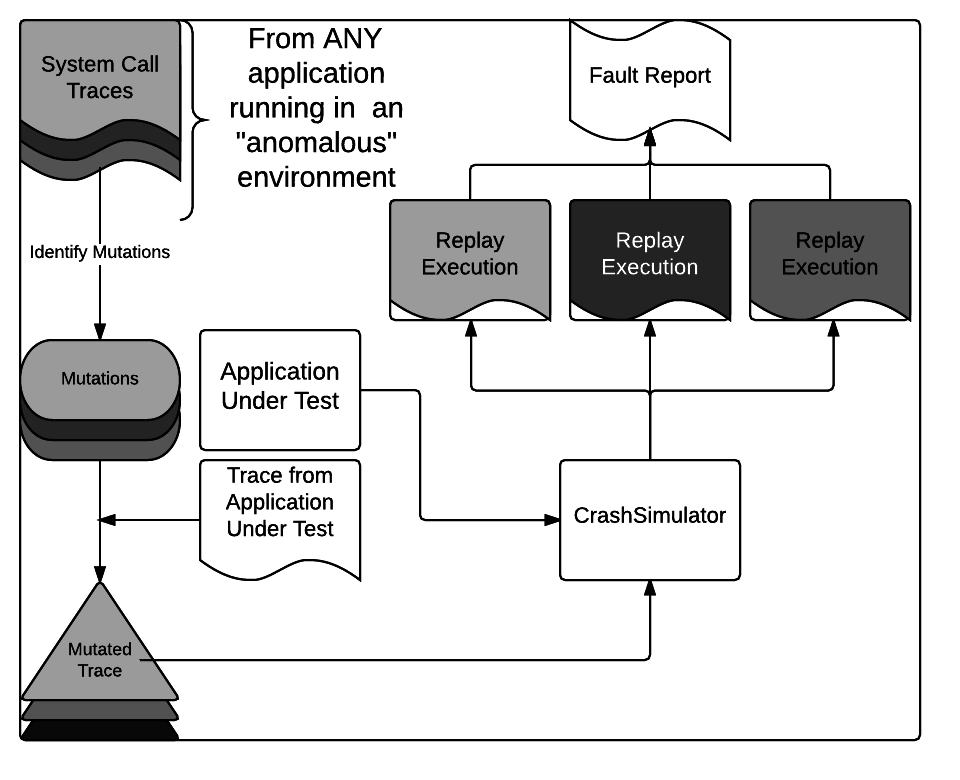
\includegraphics[scale=.5]{Architecture}}
        \caption{High level view of CrashSimulator's Architecture.}
        \label{figure:architecture}
    \end{figure}

    \preston{This is draft text from Lois.  She recommends we have a brief
      introduction on each section}  In this section, we highlight some relevant
    information behind the operation of CrashSimulator, starting with the
    rationale behind using system call traces to preserve and replay significant
    anomalies. Example of where anomalies can be found and what they resemble
    are also given, as is a description of a few key steps in its operation,
    such as the method for injecting anomalies and analyzing the execution of
    CrashSimulator’s replay process.
    
    \subsection{Rationale}

        \subsubsection{Why System Call Traces?}

        In order to inject anomalies and monitor program behavior as described
        above, CrashSimulator needs to have detailed interactions with the
        application under test at some level.  The option of carrying out these
        interactions at the system call level was chosen for several
        reasons:

        \paragraph{Tooling}

        Operating at the system call level allows this work to take advantage of
        two key pieces of tooling that already exist in mature form on Linux.
        The first is {\tt ptrace}, a process manipulation interface provided
        by the Linux kernel primarily for debugger development.
        This work leverages {\tt ptrace} in order to start and stop execution of a
        process as well as to read and write the contents of the processe's
        registers and memory.  Using these operations allows CrashSimulator to
        pause execution before and after each system call an application makes
        in order to manage execution and inject anomalies where appropriate.

        CrashSimulator also relies on system call traces recorded using {\tt
          strace}.  The {\tt strace} system call trace format is extensive and
        captures the parameters, return values, and side effects of each system
        call an application makes.  Such a record provides
        all the information needed to execute an application in
        such a way that the trace is faithfully
        replayed.  In doing so, the trace acts as an interface
        that can inject anomalous behavior into the execution of an application.

        \paragraph{Removing language dependence}

        Operating at the system call level frees CrashSimulator from
        dependence on a particular programming language, compiler, or runtime system.  
	As such, the tool does not require any complex language parsing and
        analysis code, %while still allowing it to posess many of the benefits of
        %systems that perform such work and makes it much easier to use CrashSimulator 
	so it can be used with applications written in a wide variety of languages.
	%Testing tools that perform language parsing do
	%so in order to craft inputs that specifically exercise target execution
	%paths in an application.  
	This is an important advantage as CrashSimulator is concerned with issues that arise
        at the ``interfaces'' between an application and its environment,
	and directly manipulates values at these interfaces to simulate
        %Manipulating system calls allows us to skip the process of generating
        %these crafted inputs in favor of directly effecting the
	anomalous situations of interest.

        \paragraph{Identifying Issues that Result from an Application's Environment}

        Most current testing strategies are very application-centric.  For
        example, a black box fuzzer is able to identify faults that arise when
        an application begins processing data it has received from a network
        connection. CrashSimulator, on the other hand, is able to identify
        issues that arise from the network connection itself.

    \subsubsection{Why Replay Executions?}

        Replay is important because it allows CrashSimulator to execute an
        application free from dependencies on things like file system contents,
        network configuration, or communication with other applications.  For
        example, if an application depends on a file being present in a filesystem,
        CrashSimulator can intercept calls to {\tt read()} from and {\tt write()} to
        this file, removing the need for this file to actually be present during
        replay executions. Additionally, replay allows CrashSimulator to reproduce
        the differences between versions of libraries and other executable
        dependencies, alleviating the need install them in the test environment.

    %\paragraph{Control Execution}

    %Because it is simulating aspects the application under test's environment, CrashSimulator is able to manipulate the
    %data the application receives from these aspects in order to control execution.  This is the key feature that allows
    %CrashSimulator to inject anomalous situations into an execution.  For example, by simulating the communications
    %between the application under test and another host on a network, CrashSimulator can fragment, modify, or even drop
    %data ``incoming'' from the simulated remote host in order to determine whether or not the application appropriately
    %handles the situation. 

     

    \subsection{Anomaly Identification}
    
    Prior to beginning CrashSimulator's testing
    process, we identified a set of unusual conditions (which we refer to as anomalies)
    which can be present in an environment to test against.
    This can be accomplished either manually or by
    examining results of other applications running in the target environment with existing
    tools.  This work utilized the results of both
    NetCheck~\cite{Zhuang_NSDI_2014} and CheckAPI~\cite{rasley2015detecting}, as
    well as manual analysis, to develop the set of anomalies used in our
    evaluation.  NetCheck, which can be thought of as a precursor to
    CrashSimulator, is a too that can determine the cause of a failure in a
    networked application, without any specific knowledge of the application or
    its language. It is readily able to identify a wide variety of anomalous
    behaviors related to network communication between one or more
    hosts.  CheckAPI performs a similar function by comparing the behavior of an API
    implementation to a reference model.

    Another source of anomalies is the public bug trackers of projects available
    on the web.  If the presence of a bug is indicated by a series of system
    calls, then a checker can be constructed to identify it during execution. This
    is ideal when determining whether or not an application is vulnerable to a
    widely publicized bug.  Similarly, bugs can be taken from similar projects
    in order to expand a project's set of available anomalies.

    In selecting anomalies for use it is important to understand that they
    can be as subtle as a single configuration flag being set
    differently under specific circumstances.  In BSD and OS X sockets returned
    by the {\tt accept()} system call inherit the values of the {\tt
      O\_NONBLOCK} and {\tt O\_ASYNC} flags from their parent socket.  In Linux,
    these values are not inherited.  As a result, the correct behavior is to
    always explicitly set these flags to the appropriate values on child
    sockets.  This environmental difference presented itself as a bug
    in the socket implementation of Python 3.2.  Python took advantage of
    non-blocking sockets in order to implement timeout capabilities for sockets.
    Because Python did not specifically set the {\tt O\_NONBLOCK} flag on the
    child sockets underlying its socket object abstraction, it was possible that,
    depending on the environment, the Python socket object would report the
    socket as either blocking or non-blocking while the actual underlying socket
    was configured for the opposite behavior.

    Anomalies can also be found around more complex operations.  Moving files
    around in a filesystem is an extremely common operation that, on face value,
    seems to fairly simplistic to carry out.  In reality, things become complex
    quickly once a few implementation details are taken into account: namely
    limitations in Linux's {\tt rename()} system call and the way Linux's
    directory hierarchy can abstract away complicated device configurations.

    Trivial cases of moving a file (i.e. those where the source and destination
    are on the same device) are accomplished using the {\tt rename()} system
    call.  In cases where the source and destination are not on the same device
    this system call fails and the application must handle the operation
    manually. This means that \emph{any} application that moves files around on
    a Linux system must be able to deal with the situation where some part of
    the directory structure may physically reside on a different device.
    During our evaluation, we modeled what
    it takes to move a file correctly using the GNU Coreutils {\tt mv} command
    as our ``gold standard.''  We found many applications do not handle the
    above situation correctly including the {\tt shutils} module from the Python
    2.7.9 standard library.  It did not correctly preserve timestamps across the
    move, it did not correctly apply extended file attributes to the destination
    file after the move, and it did not verify the file's inode number between
    initially examining the source file and when the copy was initiated (a
    common cause of race conditions).  Failing to perform these operations
    exposes applications relying on {\tt shutils} to misordered processing, data
    loss, or security issues.

    \subsection{Converting Anomalies to System Call Sequences}

    Once a new anomaly has been identified, it is distilled into a sequence of
    system calls that respond to the anomaly.  This process
    involves examining the system call traces %containing anomalies 
    in order to
    identify a series of calls indicative of an appropriate (or inappropriate)
    response to a specified anomaly.
    This analysis should identify two things: 1) any mutations that may need to be
    made to the trace to simulate the anomalous environment, and 2) a checker to
    examine the application's response to further trace operations in order to
    determine
    whether it is responding appropriately. These checkers can often be 
    described by finite automata, allowing CrashSimulator to simply check
    whether replay results are accepted by the automaton.

    Much like the effort involved in constructing a unit test to
    check for correct behavior in a piece of code, this
    process involves an initial outlay of user skill and effort that 
    will be paid back as it is used
    repeatedly over time.
    %Consider a Linux application that depends on a
    %particular file being present at a specific location in the filesystem.
    %If this file is usually present, a developer may forget to check the
    %return value of {\tt open ()} on it.  This will result in future calls to
    %{\tt write ()} the file failing returning -1 with {\tt errno} containing {\tt
    %EBADF} --- a result that obscures the initial cause of the failure.  The
    %key pieces of information that CrashSimulator's user must extract from
    %this situation are the true cause of the error (i.e.\ the initial open ()
    %failure) and the system call specific traits of the error (i.e.\ open ()
    %returning -1 rather than a valid file descriptor, and {\tt errno} containing
    %{\tt ENOENT}).  In come cases this step can be automated (consider NetCheck
    %automatically diagnosing some classes of network-related errors) but in
    %other cases manual effort will be required.}

    With this information in mind, a developer can construct the simple
    mutation ``make the {\tt open ()} call return -1 with {\tt errno} set to
    {\tt ENOENT}'' and use CrashSimulator to apply it to any application that
    makes {\tt open ()} calls.  Using these mutated traces can allow
    CrashSimulator to perform a universal test for whether or not an
    application correctly checks {\tt open()}'s return value.

    %CrashSimulator can use the outputs of this analysis either as mutations to
    %be applied to a system call trace of the application under test or as input
    %to a ``checker'' that determines whether an application has performed a
    %required set of actions. When a ``checker'' is required, the sequence of
    %system calls is encoded as a finite automaton that, when provided with as
    %input the system calls made during the course of a replay execution, can
    %decide whether or the pattern of system calls is present.  If the analysis
    %reveals that anomalous conditions need to be injected into a replay
    %execution this is facilitated by modifying the to-be-replayed system call
    %trace from the application under test.

    In some cases, %only one of these pieces is required for CrashSimulator to
   % perform its analysis. 
    the checker is very simple and in others it is more complex.
   % If there is not a definite correct response system
   % call sequence,
   In many situations
    CrashSimulator's default checker can be employed to determine
    whether the application has noticed the anomaly and whether it may be making
    an effort to handle it (See example in
    \S~\ref{sec-file-type-bugs}).  From the other direction,
    the system can employ more specific checkers in a replay execution 
    to determine whether the application handled
    all the edge cases.  We employed this technique in our
    evaluation of CrashSimulator's ability to find bugs related to moving files across
    devices (\S~\ref{sec-complex}).
    
    \subsection{Anomaly Injection}

    CrashSimulator's replay-based approach makes it easy to inject anomalies
    into an execution.  
    Because its execution faithfully
    follows the system call behavior described in the trace being
    replayed, anomalous behavior can be introduced either by modifying
    this trace manually or programmatically.
    For example, suppose an anomaly causes a
    call to {\tt read()} fail with return value of -1 and {\tt errno} set to
    {\tt EINVAL}.  Exposing an application to this situation only requires
    editing the system call trace, such that the line describing this read call
    reflects the above values.

    %Consider the example of an anomaly identified in a web server application.
    %This behavior can distilled down to a series of system calls indicitive of
    %the anomaly.  If this behavior is present in other network-reliant
    %applications it too can be identified by looking for the same series of
    %system calls.  This series of system calls can then be transformed into a
    %computational model as described above.  As another example, consider the
    %bugs in Python's shutils that were discussed earlier.  In the case of the
    %``race condition'' bug, the series of system calls indicative of its
    %presence is an application using stat() to check a file, open() to open it,
    %and a series of read() and write() calls to copy its contents to the
    %destination without a call to fstat() that to confirm that the file was not
    %modified after the initial call to stat().


    \subsection{Analyzing an Execution}

    CrashSimulator's replay process consists of launching the
    application under test as a child process and interceeding in its execution
    at appropriate times in order to simulate the results and side effects of any
    system call the application might make.
    The trace is mutated to reflect the chosen anomaly, ensuring the process
    will reveal the anomaly to the application.
    After the replayed execution
    concludes, CrashSimulator is able to use the ending state of the checker to
    report whether or not the anomalous situation was handled appropriately.
    CrashSimulator
    can use two types of checkers, which each serve a slightly different purpose.

    %The up front effort
    %in this process only needs to be done once. One of CrashSimulator's major
    %advantges over application-specific test suites is that checkers and, if
    %necessary, any associated system call trace mutations can be accumulated and
    %used to test any application CrashSimulator's user is interested in.

    %In the case of the Python
    %shutils race condition, the faulty behavior can be identified using a simple
    %python script that calls shutils.move() to move a file between directories
    %located on different storage devices.  CrashSimulator is able to identify
    %the bad behavior by replaying a system call trace taken of an execution of
    %the Python interpreter while it executes the script in question.

    %For example, a set of bugs that will be
    %discussed later were found by modifying a rename() system call to return a
    %result indicating that the application is attempting to move a file across
    %disks -- an operation the system call cannot perform.  In a well behaved
    %application, this will trigger an alternative execution path wherein the
    %file is manually copied by the application.  In a buggy application either
    %this case will be handled incorrectly (i.e. the appliation will fail to
    %perform all of the steps required to properly copy a file across devices, a
    %situation caught by well-constructed anomaly models) or will not be handled
    %at all, that is, the application will fail eventually because it did not
    %recognize that the call to rename was not successful.

    %I feel like this is important to include but am having trouble figuring out
    %where to put it.
    
    \paragraph{The Default Checker}

    When CrashSimulator injects anomalous behavior into a replay execution it is
    expected that the application under test will deal with this
    anomaly in some way. For example, applications
    can be expected to behave differently when
    the structure returned by a call to {\tt stat()} indicates the target file
    is a symlink, rather than a regular file.
    When there are numerous ways an
    application could correctly handle a given anomaly, CrashSimulator 
    can use a generic ``default checker''.  This default checker
    is based on the assumption that an application's efforts to deal with the anomaly
    will result in it executing different program paths (and therefore different
    system calls) than were executed when the system call trace
    was recorded.  If the application being replayed does not
    alter its behavior to deal with the anomaly, it has not
    correctly handled this flaw --- a failing result.  Alternatively, if the
    application does deviate,
    it is likely that the application is taking some action
    to handle the injected condition --- an indication of possibly correct
    behavior.

    This approach is often sufficient to classify application behavior. % because in reality, 
    %a test can only tell us if
    %an application performs a specific bad behavior in a specific situation.  A
    %test cannot prove that an application is bug free in the same situation. 
    As
    with traditional tests, CrashSimulator does not tell us that an application is
    bug free in a given situation; instead, it asserts that an application
    has incorrectly handled a given situation.
    

    \paragraph{More Specific Checkers}

    CrashSimulator also accepts more specific checkers that evaluate whether or
    not an application has performed a required operation.  These checkers
    monitor a replay execution for a specific system call sequence (with the
    correct parameters, return values, and state modifications) that indicates
    the application has carried out the operation in question.  To achieve this,
    these checkers use a model (e.g. a deterministic finite
    automaton, a push down automaton, etc.) that accepts particular system
    call sequences indicative of correct (or incorrect) response
    to the anomaly.  Whether CrashSimulator
    ultimately accepts a given replay execution is determined by the ending
    states of the checkers monitoring the execution.


%    These deficiencies are not just inconveniences.  They can have a real world
%    impact on a system's operation and security.  Consider the case of not
%    correctly copying timestamps when when moving a file.  If other code depends
%    on timestamps for ordering its processing then moving the file via {\tt
%      shutils} can result in a silent mis-ordering of its processing.  This
%    could be disaster in order-dependent situations like batching updates to a
%    database.  Additionally, failing to confirm a file's inode before moving can
%    result in data loss or security issues if the file is replaced in the middle
%    of the copy process.  Further, failing to copy extended
%    file attributes to a destination file can result in the operating system
%    mishandling trust concers around an untrusted file.

    \subsection{CrashSimulator Architecture}
        
    At a high level CrashSimulator is organized into two primary modules. The
    first is responsible for monitoring a given execution, determining
    when to inject anomalous behavior, and if the
    application responded correctly.  The second module
    is responsible for managing the execution of the application under test such
    that it precisely follows a previously recorded system call trace -- a
    process we refer to as ``replaying'' a system call trace.

    %The first step in CrashSimulator's work flow is to identify anomalous behavior in an arbitrary application.
    %Currently, this step is accomplished through manual bug hunting and through examination of diagnostic output from
    %NetCheck and CheckAPI. CrashSimulator's user examines the system call behavior that resulted in this bad behavior
    %and constructs a model that defines what triggers the anomalous behavior and the subsequent ``bad'' system call
    %behavior (\emph{Do we need to say something about future work doing this step automatically here?}.
    %CrashSimulator's first module operates by using this model to analyzed the system call behavior of the application
    %under test(e.g. order, parameters, side effects, return values).
        
    Both modules make use of the {\tt ptrace} facilities built into modern
    versions of the Linux kernel.  A ``replay''
    is achieved by intercepting key system calls made by the application,
    preventing the call from being carried out by the kernel (by
    converting it to a call to {\tt getpid()}), identifying the matching system
    call from a previously recorded trace, and replicating the return value
    and side effects. In doing so, the application believes that the system call it
    made actually took place. We have found that emulating the post conditions
    of a system call results in faithful replays of a
    previous execution in most cases.

    CrashSimulator is fully self contained and operates without user
    intervention during its analysis process. At this point, the tool 
    itself is available as a virtual machine appliance that is compatible with the
    \emph{Virtual Box} virtual machine hosting software.  The decision to
    distribute CrashSimulator in this manner is based on three points.  First, this
    distribution method ensures that all of CrashSimulator's dependences are
    installed and configured appropriately.  Second, it provides an
    environment for taking system call traces that is known to be complete
    tool-wise and compatible.  Finally, and most importantly,
    this method provides an environment that is known to be compatible with the
    details of CrashSimulator's system call replay techniques.

    CrashSimulator's source code is available and, while other environments may
    be untested, it should function correctly on any platform that meets the
    criteria described above.
